\documentclass{beamer}
\mode<presentation>
\usepackage{amsmath,amssymb,mathtools}
\usepackage{textcomp}
\usepackage{gensymb}
\usepackage{adjustbox}
\usepackage{subcaption}
\usepackage{enumitem}
\usepackage{multicol}
\usepackage{listings}
\usepackage{url}
\usepackage{graphicx} % <-- needed for images
\def\UrlBreaks{\do\/\do-}

\usetheme{Boadilla}
\usecolortheme{lily}
\setbeamertemplate{footline}{
  \leavevmode%
  \hbox{%
  \begin{beamercolorbox}[wd=\paperwidth,ht=2ex,dp=1ex,right]{author in head/foot}%
    \insertframenumber{} / \inserttotalframenumber\hspace*{2ex}
  \end{beamercolorbox}}%
  \vskip0pt%
}
\setbeamertemplate{navigation symbols}{}

\lstset{
  frame=single,
  breaklines=true,
  columns=fullflexible,
  basicstyle=\ttfamily\tiny   % tiny font so code fits
}

\numberwithin{equation}{section}

% ---- your macros ----
\providecommand{\nCr}[2]{\,^{#1}C_{#2}}
\providecommand{\nPr}[2]{\,^{#1}P_{#2}}
\providecommand{\mbf}{\mathbf}
\providecommand{\pr}[1]{\ensuremath{\Pr\left(#1\right)}}
\providecommand{\qfunc}[1]{\ensuremath{Q\left(#1\right)}}
\providecommand{\sbrak}[1]{\ensuremath{{}\left[#1\right]}}
\providecommand{\lsbrak}[1]{\ensuremath{{}\left[#1\right.}}
\providecommand{\rsbrak}[1]{\ensuremath{\left.#1\right]}}
\providecommand{\brak}[1]{\ensuremath{\left(#1\right)}}
\providecommand{\lbrak}[1]{\ensuremath{\left(#1\right.}}
\providecommand{\rbrak}[1]{\ensuremath{\left.#1\right)}}
\providecommand{\cbrak}[1]{\ensuremath{\left\{#1\right\}}}
\providecommand{\lcbrak}[1]{\ensuremath{\left\{#1\right.}}
\providecommand{\rcbrak}[1]{\ensuremath{\left.#1\right\}}}
\theoremstyle{remark}
\newtheorem{rem}{Remark}
\newcommand{\sgn}{\mathop{\mathrm{sgn}}}
\providecommand{\abs}[1]{\left\vert#1\right\vert}
\providecommand{\res}[1]{\Res\displaylimits_{#1}}
\providecommand{\norm}[1]{\lVert#1\rVert}
\providecommand{\mtx}[1]{\mathbf{#1}}
\providecommand{\mean}[1]{E\left[ #1 \right]}
\providecommand{\fourier}{\overset{\mathcal{F}}{ \rightleftharpoons}}
\providecommand{\system}{\overset{\mathcal{H}}{ \longleftrightarrow}}
\providecommand{\dec}[2]{\ensuremath{\overset{#1}{\underset{#2}{\gtrless}}}}
\newcommand{\myvec}[1]{\ensuremath{\begin{pmatrix}#1\end{pmatrix}}}
\let\vec\mathbf

\title{MatGeo Presentation - Problem 11.2.5}
\author{EE25BTECH11064 - Yojit Manral}
\date{}

\begin{document}

\frame{\titlepage}
\begin{frame}{Question}
In $\triangle ABC$, $\vec{D}$, $\vec{E}$ and $\vec{F}$ are, respectively, the mid-points of sides AB, BC and CA. Show that $\triangle ABC$ is divided into four congruent triangles by joining $\vec{D}$, $\vec{E}$, and $\vec{F}$.
\end{frame}

\begin{frame}{Solution}
$\rightarrow$ Given that
\begin{align}
    \vec{D} = \frac{\vec{A}+\vec{B}}{2} && \vec{E} = \frac{\vec{B}+\vec{C}}{2} && \vec{F} = \frac{\vec{C}+\vec{A}}{2}
\end{align}
$\rightarrow$ From (1), it follows that
\begin{align}
    \vec{A} = \vec{D}+\vec{F}-\vec{E} && \vec{B} = \vec{E}+\vec{D}-\vec{F} && \vec{C} = \vec{F}+\vec{E}-\vec{D}
\end{align}
$\rightarrow$ From (2), we get that
\begin{align}
    \text{In }\triangle FAD\text{ and }\triangle DEF \\
    \vec{A}-\vec{D} = \vec{F}-\vec{E}\text{ (Side 1)} \\
    \vec{A}-\vec{F} = \vec{D}-\vec{E}\text{ (Side 2)} \\
    \vec{D}-\vec{F}\text{ is common to both} \\
    \triangle FAD \cong \triangle DEF\text{(SSS criterion)}
\end{align}
\end{frame}

\begin{frame}{Solution}
\begin{align}
    \text{In }\triangle DBE\text{ and }\triangle DEF \\
    \vec{B}-\vec{E} = \vec{D}-\vec{F}\text{ (Side 1)} \\
    \vec{B}-\vec{D} = \vec{E}-\vec{F}\text{ (Side 2)} \\
    \vec{E}-\vec{D}\text{ is common to both} \\
    \triangle DBE \cong \triangle DEF\text{(SSS criterion)}
\end{align}
\begin{align}
    \text{In }\triangle ECF\text{ and }\triangle DEF \\
    \vec{C}-\vec{F} = \vec{E}-\vec{D}\text{ (Side 1)} \\
    \vec{C}-\vec{E} = \vec{F}-\vec{D}\text{ (Side 2)} \\
    \vec{F}-\vec{E}\text{ is common to both} \\
    \triangle ECF \cong \triangle DEF\text{(SSS criterion)}
\end{align}
$\rightarrow$ From (7), (12), and (17), we know that $\triangle ABC$ is divided into four congruent triangles
\end{frame}

\begin{frame}{Solution}
\begin{align}
    \triangle FAD \cong \triangle DBE \cong \triangle ECF \cong \triangle DEF
\end{align}
\begin{figure}[h!]
   \centering
   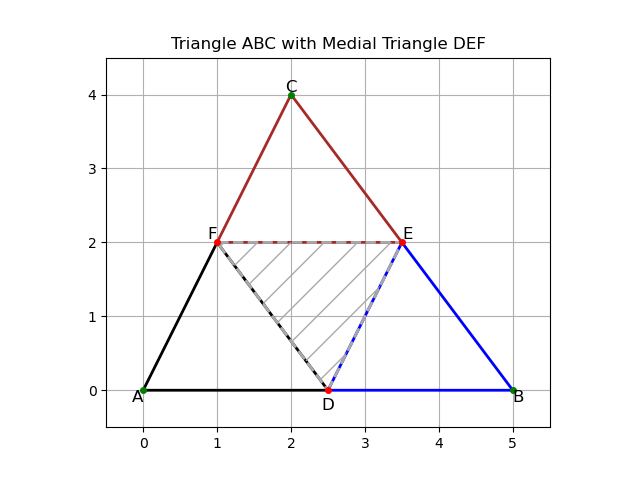
\includegraphics[width=0.65\linewidth]{figs/01.png}
   \caption{Plot of $\triangle ABC$ and its medial triangle $\triangle DEF$}
   \label{Plot_1}
\end{figure}
\end{frame}
 % --------- CODE APPENDIX ---------
\section*{Appendix: Code}
% Python plotting
\begin{frame}[fragile]{File: plot.py}
\begin{lstlisting}[language=Python]
import matplotlib.pyplot as plt
import numpy as np

# Coordinates of the vertices of triangle ABC
A = np.array([0, 0])
B = np.array([5, 0])
C = np.array([2, 4])
# Midpoints of the sides
D = (A + B) / 2
E = (B + C) / 2
F = (C + A) / 2

# Plot the triangle ABC
fig, ax = plt.subplots()
triangle1 = plt.Polygon([A, D, F], fill=None, edgecolor='black', linewidth=2, zorder=2)
triangle2 = plt.Polygon([B, E, D], fill=None, edgecolor='blue', linewidth=2, zorder=2)
triangle3 = plt.Polygon([C, F, E], fill=None, edgecolor='brown', linewidth=2, zorder=2)
triangle4 = plt.Polygon([D, E, F], fill=None, edgecolor='darkgray', hatch='/', linestyle='--', linewidth=2, zorder=2)

# Plotting the triangle ABC and medial triangle DEF
ax.add_patch(triangle1)
ax.add_patch(triangle2)
ax.add_patch(triangle3)
ax.add_patch(triangle4)
\end{lstlisting}
\end{frame}

\begin{frame}[fragile]{File: plot.py}
\begin{lstlisting}[language=Python]
# Plot the points A, B, C, D, E, F
ax.plot(A[0], A[1], 'go', ms=4)  # A
ax.plot(B[0], B[1], 'go', ms=4)  # B
ax.plot(C[0], C[1], 'go', ms=4)  # C
ax.plot(D[0], D[1], 'ro', ms=4)  # D
ax.plot(E[0], E[1], 'ro', ms=4)  # E
ax.plot(F[0], F[1], 'ro', ms=4)  # F

# Labels for points
ax.text(A[0], A[1], 'A', fontsize=12, ha='right', va='top')
ax.text(B[0], B[1], 'B', fontsize=12, ha='left', va='top')
ax.text(C[0], C[1], 'C', fontsize=12, ha='center', va='bottom')
ax.text(D[0], D[1]-0.1, 'D', fontsize=12, ha='center', va='top')
ax.text(E[0], E[1], 'E', fontsize=12, ha='left', va='bottom')
ax.text(F[0], F[1], 'F', fontsize=12, ha='right', va='bottom')

# Title and showing the plot
ax.set_aspect('equal')
ax.grid()
plt.xlim(-0.5, 5.5)
plt.ylim(-0.5, 4.5)
plt.title("Triangle ABC with Medial Triangle DEF")
plt.show()
\end{lstlisting}
\end{frame}

\end{document}
